%chktex-file 1

\section{\large Ejercicio 1: Axiomas en un Espacio Vectorial.}
Realice la verificación de los siguientes axiomas del espacio vectorial $\mathbf{R}^3$ utilizando los escalares y los vectores proporcionados.

\[
    \text{\textit{Vectores: }}\vec{u}=(8,4,-3);\vec{v}=(1,-9,7)\text{ y }\vec{w}=(-3,-8,8)
\]
\[
    \text{\textit{Escalares: }}\lambda=7;\beta=2
\]


\begin{itemize}
    \item Cerradura bajo la suma de vectores: \(\text{\textit{Si} }\vec{u},\vec{v}\in\mathbb{R}^3,\text{ \textit{entonces} }\vec{u}+\vec{v}\in\mathbb{R}^3\).
    \[
        \vec{u}+\vec{v}=(9,-5,4)
    \]
    \begin{figure}[ht!]
        \centering
        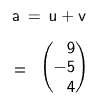
\includegraphics[width=100pt,height=100pt]{img/imagen1.png}
        \caption{Comprobación en GeoGebra}
    \end{figure}

    \item Cerradura bajo el producto escalar: \(\text{\textit{Si} }\lambda\in\mathbb{R}^3\text{ y }\vec{u}\in\mathbb{R}^3,\text{ \textit{entonces} }\lambda\vec{u}\in\mathbb{R}^3\)
    
    \[
        7(8,4,-3)=(56,28,-21)
    \]
    \begin{figure}[ht!]
        \centering
        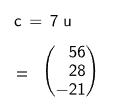
\includegraphics[width=100pt,height=100pt]{img/imagen2.png}
        \caption{Comprobación en GeoGebra}
    \end{figure}

    \item Asociatividad de la suma: \(\vec{u}+(\vec{v}+\vec{w})=(\vec{u}+\vec{v})+\vec{w}\)
    
    \[
        \vec{u}+(\vec{v}+\vec{w})
    \]
    \[
        (8,4,-3)+(-2,-17,15)=(6-13,12)
    \]
    \[
        (\vec{u}+\vec{v})+\vec{w}
    \]
    \[
        (9,-5,4)+(-3,-8,8)=(6,-13,12)
    \]

    \begin{figure}[ht!]
        \centering
        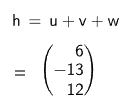
\includegraphics[width=100pt,height=100pt]{img/imagen3.png}
        \caption{Comprobación en GeoGebra}
    \end{figure}

    \item Existencia de elemento neutro aditivo: \(\vec{u}+\vec{0}=\vec{0}+\vec{u}=\vec{u}\)
    

    \[
        (8,4,-3)+(0,0,0)=(8,4,-3)
    \]
    \[
        (0,0,0)+(8,4,-3)=(8,4,-3)
    \]

    \begin{figure}[ht!]
        \centering
        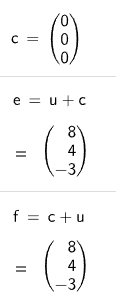
\includegraphics[width=100pt,height=200pt]{img/imagen4.png}
        \caption{Comprobación en GeoGebra}
    \end{figure}

    \item Existencia de inverso aditivo: \(\vec{u}+(-\vec{u})=(-\vec{u})+\vec{u}=\vec{0}\)
    
    \[
        \vec{u}+(-\vec{u})
    \]
    \[
        (8,4,-3)+(-8,-4,3)=(0,0,0)
    \]
    \[
        (-\vec{u})+\vec{u}
    \]
    \[
        (-8,-4,3)+(8,4,-3)=(0,0,0)
    \]

    \begin{figure}[ht!]
        \centering
        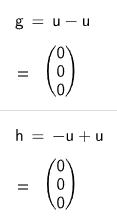
\includegraphics[width=100pt,height=200pt]{img/imagen5.png}
        \caption{Comprobación en GeoGebra}
    \end{figure}

    \FloatBarrier
    \item Conmutatividad de la suma: \(\vec{u}+\vec{v}=\vec{v}+\vec{u}\)
    
    \[
        (8,4,-3)+(1,-9,7)=(9,-5+4)
    \]
    \[
        (1,-9,7)+(8,4,-3)=(9,-5+4)
    \]

    \begin{figure}[ht!]
        \centering
        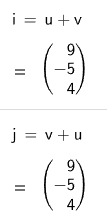
\includegraphics[width=100pt,height=200pt]{img/imagen6.png}
        \caption{Comprobación en GeoGebra}
    \end{figure}
    
    \FloatBarrier
    \item Asociatividad de la multiplicación por escalar: \((\lambda\beta)\vec{u}=\lambda(\beta\vec{u})\)
    
    \[
        14(8,4,-3)=(112,56,-42)
    \]
    \[
        7(16,8,-6)=(112,56,-42)
    \]

    \begin{figure}[ht!]
        \centering
        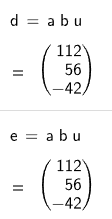
\includegraphics[width=100pt,height=200pt]{img/imagen7.png}
        \caption{Comprobación en GeoGebra}
    \end{figure}

    \FloatBarrier
    \item Distributividad a derecha de la multiplicación escalar con respecto a la suma de vectores: \(\lambda(\vec{u}+\vec{v})=\lambda\vec{u}+\lambda\vec{v}\)
    
    \[
        \lambda(\vec{u}+\vec{v})
    \]
    \[
        7(9,-5,4)=(63,-35,28)
    \]
    \[
        \lambda\vec{u}+\lambda\vec{v}
    \]
    \[
        (56,28,-21)+(7,-63,49)=(63,-37,28)
    \]
    \begin{figure}[ht!]
        \centering
        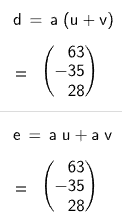
\includegraphics[width=100pt,height=200pt]{img/imagen8.png}
        \caption{Comprobación en GeoGebra}
    \end{figure}

    \FloatBarrier
    \item Distributividad de la multiplicación escalar con respecto a la suma de escalares: \((\lambda+\beta)\vec{u}=\lambda\vec{u}+\beta\vec{u}\)
    
    \[
        \lambda+\beta\vec{u}
    \]
    \[
        9(72,36,-27)
    \]
    \[
        \lambda\vec{u}+\beta\vec{u}
    \]
    \[
        (56,28,-21)+(16,8,-6)=(72,36,-27)
    \]
    \begin{figure}[ht!]
        \centering
        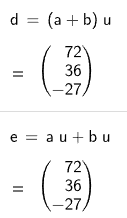
\includegraphics[width=100pt,height=200pt]{img/imagen9.png}
        \caption{Comprobación en GeoGebra}
    \end{figure}
\end{itemize}